%%%%%%%%%%%%%%%%%%%%%%%%%%%%%%%%%%%%%%%%%%%%%%%%%%%%%%%%%%%%%%%%%%%%%
% PREAMBLE
%%%%%%%%%%%%%%%%%%%%%%%%%%%%%%%%%%%%%%%%%%%%%%%%%%%%%%%%%%%%%%%%%%%%%
%
% The following two commands will generate a PDF that follows all the requirements for submission
% and peer review.  Uncomment these commands to generate this output (and comment out the two lines below.)
%
% DOUBLE SPACE VERSION FOR SUBMISSION TO THE AMS
\documentclass[12pt]{article}
\usepackage{ametsoc}
%
% The following two commands will generate a single space, double column paper that closely
% matches an AMS journal page.  Uncomment these commands to generate this output (and comment
% out the two lines above. FOR AUTHOR USE ONLY. PAPERS SUBMITTED IN THIS FORMAT WILL BE RETURNED
% TO THE AUTHOR for submission with the correct formatting.
%
% TWO COLUMN JOURNAL PAGE LAYOUT FOR AUTHOR USE ONLY
%%%%\documentclass[10pt]{article}
%%%%\usepackage{ametsoc2col}
%
%%%%%%%%%%%%%%%%%%%%%%%%%%%%%%%%%%%%%%%%%%%%%%%%%%%%%%%%%%%%%%%%%%%%%
% ABSTRACT
%
% Enter your Abstract here
%%%%%%%%%%%%%%%%%%%%%%%%%%%%%%%%%%%%%%%%%%%%%%%%%%%%%%%%%%%%%%%%%%%%%
\newcommand{\myabstract}{
Direct calculations of the entrainment and detrainment of air between
clouds and their environment require a knowledge of the relative velocity
difference between the air and the cloud surface. LES model grids
force the distance moved by the cloud surface over a timestep to be
either zero or the width of a model grid cell, while in reality the
cloud surface tends to move at a more constant rate. Here we present
a method for the subgrid interpolation of a cloud surface given total
humidity and saturated humidity on a regular LES grid. This method
is used to calculate entrainment and detrainment rates for an LES
model, which are compared with rates inferred from bulk conserved
tracer calculations.  Our method agrees well with bulk tracer calculations of 
entrainment and detrainment if the bulk tracer calculations are corrected to
account for the influence of the moist cloud shell.
}
%
\begin{document}
%
%%%%%%%%%%%%%%%%%%%%%%%%%%%%%%%%%%%%%%%%%%%%%%%%%%%%%%%%%%%%%%%%%%%%%
% TITLE
%
% Enter your TITLE here
%%%%%%%%%%%%%%%%%%%%%%%%%%%%%%%%%%%%%%%%%%%%%%%%%%%%%%%%%%%%%%%%%%%%%
\title{\textbf{\large{Interpolation of LES cloud surfaces for use in direct
calculations of entrainment and detrainment}}}
%
% Author names, with corresponding author information. 
% [Update and move the \thanks{...} block as appropriate.]
%
\author{\textsc{Jordan T. Dawe}
	\thanks{\textit{Corresponding author address:} 
	Jordan T. Dawe, Department of Earth and Ocean Sciences, University of British Columbia 
	6339 Stores Road, Vancouver, BC, V6T 1Z4. 
	\newline{E-mail: jdawe@eos.ubc.ca}}\quad\textsc{and Phillip Austin}\\
\textit{\footnotesize{Department of Earth and Ocean Sciences, University of British Columbia, Vancouver, BC}}
\and 
\centerline{\textsc{Extra Author}}\\% Add additional authors, different insitution
\centerline{\textit{\footnotesize{Affiliation, City, State/Province, Country}}}
}
%
% Formatting done here...Authors should skip over this.  See above for abstract.
\ifthenelse{\boolean{dc}}
{
\twocolumn[
\begin{@twocolumnfalse}
\amstitle

% Start Abstract (Enter your Abstract above.  Do not enter any text here)
\begin{center}
\begin{minipage}{13.0cm}
\begin{abstract}
	\myabstract
	\newline
	\begin{center}
		\rule{38mm}{0.2mm}
	\end{center}
\end{abstract}
\end{minipage}
\end{center}
\end{@twocolumnfalse}
]
}
{
\amstitle
\begin{abstract}
\myabstract
\end{abstract}
}
%%%%%%%%%%%%%%%%%%%%%%%%%%%%%%%%%%%%%%%%%%%%%%%%%%%%%%%%%%%%%%%%%%%%%
% MAIN BODY OF PAPER
%%%%%%%%%%%%%%%%%%%%%%%%%%%%%%%%%%%%%%%%%%%%%%%%%%%%%%%%%%%%%%%%%%%%%

\section{Introduction}

The largest uncertainties in Global Circulation Model (GCM) simulations
come from the subgridscale parameterization of clouds. The IPCC 2007
report found the *TK* models they examined showed a *TK* W
m$^{-2}$ range in the cloud feedback response, relative to a *TK*
W m$^{-2}$ total climate sensitivity.  Improvements in the accuracy of 
these subgridscale cloud parametrizations are neccessary to simulate 
the spatial pattern and rate of global warming.

Proper simulation of the subgridscale effect of cumulus clouds in
GCMs requires understanding the rates at which air is entrained into
and detrained from the clouds. Cloud entrainment and detrainment rates
exert influences on profiles of cloud properties, the height of the
cloud tops, the amount of heat and moisture the clouds transport upwards,
and the heights at which the clouds deposit that heat and moisture.
They also have effects on the vertical transport of aerosols out of
the boundary layer and the rate at which chemical reactions can occur
in those aerosols. Several approaches to the parametrization of entrainment
and detrainment rates have been proposed, including *TK*.

Large Eddy Simulation (LES) is an important tool used in the study
of cloud entrainment and detrainment. LES models achieve grid resolutions
on the order of 10-100 m, so that the smallest length scales resolved
by the model touch the small wave number end of the Kolmagorov -5/3
turbulence spectrum. This allows for a relatively simple turbulence
model that captures the important statistics of the subgridscale eddy
fluxes and thus, an accurate representation of the atmospheric physics
of a domain \textasciitilde{}10 km$^{2}$, which is enough to simulate
a field of clouds. LES simulations can be ground-truthed against results
taken from large field surveys, such as the Barbados Oceanographic
and Meteorological Experiment (BOMEX) or the Atmospheric Radiation
Measurement (ARM) Program, and such comparisons show good agreement
between the LES simulations and field data.

Several recent studies have looked at the lifecycle of individual
clouds taken from LES models, trying to break the cloud field into
its component parts. Estimates of entrainment and detrainment rates
for individual clouds would be quite useful in these types of studies,
but are difficult to achieve. Entrainment and detrainment rates are 
typically calculated in LES simulations by recording budgets
of bulk conserved tracer variables, such as the total humidity or
the liquid water moist static energy, and inferring the amount of
fluid exchange between cloud and clear air that is needed to explain
the rate at which that tracer is being vertically advected within
the cloud field. These budgets typically assume the clouds and the
cloud environment are horizontally homogenous slabs; this is a much
less accurate assumption on the level of an individual cloud.

Alternatively, entrianment and detrianment could simply be calculated
directly from the LES velocity and humidity field.  \cite{Siebesma1998} 
defines Entrainment and Detrainment as

\begin{equation}
E = -\frac{1}{A}\oint_{\mathbf{\hat{n}}\cdot(\mathbf{u} - \mathbf{u_i}) < 0}
\mathbf{\hat{n}}\cdot(\mathbf{u}-\mathbf{u_i})dl
\end{equation}
\begin{equation}
D = \frac{1}{A}\oint_{\mathbf{\hat{n}}\cdot(\mathbf{u} - \mathbf{u_i}) > 0}
\mathbf{\hat{n}}\cdot(\mathbf{u}-\mathbf{u_i})dl
\end{equation}

where $E$ and $D$ are the entrainment and detrainment rates in kg 
m$^{-3}$ s$^{-1}$, u is velocity in m s$^{-1}$, *TK*.  However, the
accuracy of this method suffers from the need to calculate the velocity 
of the air relative to the cloud surface.  In reality 
these velocities are very nearly identical, \textasciitilde{} 1 m 
s$^{-1}$, but the discrete nature of the LES model grid forces the 
modeled surface velocity to be either 0 m s$^{-1}$ or $\Delta x / \Delta t 
\approx$ 30 m s$^{-1}$, where $\Delta x$ is the model grid spacing and 
$\Delta t$ is the model timestep.  The surface of the cloud only moves 
when a grid cell's humidity reaches saturation, and when it 
does, an entire grid cell worth of fluid leaves or enters the cloud.  This 
causes both the entrainment and detrainment to be over-estimated.

Here we present a method for calculation of the cloud entrainment and 
detrainment rates that relies on interpolation of the subgrid location 
of the cloud surface.  In section 2 we describe this method, in section 
3 we compare this calculation with entrainment and detrainment rates 
calculated using bulk conserved tracer budgets, and in section 4 we 
discuss our results.  With this method, we believe accurate estimates 
of the cloud entrainment and detrainment rates are possible for 
individual LES clouds.

%==============================================================================

\section{Method}

\subsection{Flux Calculations}

Consider a 3-d numerical model grid cell (Figure \ref{fig:cell_diagram}) 
containing a cloud surface $\mathbf{A}$, where the vectors representing 
$\mathbf{A}$ point outward from the cloud.  For the moment we neglect 
specifying the interpolation scheme that determines this surface.  This 
surface, combined with the walls of the grid cell, encloses a cloud volume $V$.

Converted to our notation, \cite{Siebesma1998} gives the net Entrainment 
and Detrainment over the cloud interface to be:

\begin{equation}
\label{eq:E_minus_D} 
E - D = \int_A \rho ( \mathbf{u} -  \mathbf{u_i}) \cdot d\mathbf{A}.
\end{equation}

where $\rho$ is the air density in kg m$^{-3}$, $\mathbf{u}$ is the velocity
of the air in m s$^{-1}$ and $\mathbf{u_i}$ is the velocity of the cloud 
interface. Calculating this integral for a numerical model cloud field would 
require interpolation of the velocity field to the surface of $\mathbf{A}$ and 
a record of the time evoluion of $\mathbf{A}$.  Instead, we seek a simplified 
but equivalent calculation.

To calculate the velocity of the cloud interface, we make use of the Leibnitz 
Theorem:

\begin{equation}
\label{eq:leibnitz} 
\frac{d}{dt}\int_{V(t)} \rho dV = 
  \int_{V(t)} \frac{\partial \rho}{ \partial t} dV 
  + \int_{A(t)} \rho \mathbf{u_i}\cdot d\mathbf{A}
\end{equation}

If we assume ${\partial \rho}/{ \partial t} \approx 0$, we can combine 
equations (\ref{eq:E_minus_D}) and (\ref{eq:leibnitz}) to give:

\begin{equation}
E - D = \rho \int_A \mathbf{u} \cdot d\mathbf{A} 
      - \rho \frac{d}{dt}\int_{V(t)} dV.
\end{equation}

Next we apply the divergence theorem to simplify the flux integral through 
$\mathbf{A}$:

\begin{equation}
\label{eq:divergence} 
\int_{V} \nabla \cdot (\rho \mathbf{u}) dV = 
  \int_{A} \rho \mathbf{u}\cdot d\mathbf{A}
\end{equation}

Due to mass conservation, $\nabla \cdot (\rho \mathbf{u}) = 0$, which implies 
that the massflux passing through $\mathbf{A}$ is equal to the massflux 
entering the volume $V$ through the walls of the model grid cell.  Since model 
continuity equations generally assume that u and v velocities are constants 
over a given grid cell wall, we calculate these fluxes simply by multiplying 
the velocity by the area of the grid cell wall occupied by cloud.  This is 
trivial for a model using an Arakawa C-grid, while interpolation can give 
velocities at the grid cells for other grid configurations.  This results in

\begin{equation}
\label{eq:entrainment_detrainment} 
E - D = \rho \int_S \mathbf{u} \cdot d\mathbf{S} - \rho \frac{dV}{dt}
\end{equation}.

Therefore, to calculate the entrainment and detrainment, we need to calculate 
the mass flux through the cloudy portion of the grid cell walls and the rate of 
change of the cloud volume inside the grid cell.  This technique will work 
equally well for flux through any surface, such as the cloud core entrainment 
and detrainment.  For simplicity we only record the net entrainment or 
detrainment in each grid cell, so if equation 
(\ref{eq:entrainment_detrainment}) is greater than zero, the total is applied 
to entrainment and if less than zero, to detrainment.

%-----------------------------------------------------------------------------

\subsection{Cloud Surface Interpolation}

There are a multitude of interpolation schemes that can be used to determine 
the cloud volume and cell wall area in a numerical model.  The simplest would 
be to assume that saturated grid cells are completely filled with cloud and 
unsaturated grid cells have no cloud at all.  We refer to this as the "no 
interpolation" case.  Since the cloud surface only moves when a whole grid cell 
undergoes condensation or evaporation, this will result in poor estimates of 
$dV/dt$ and $\mathbf{S}$, which will then overestimate the entrainment and 
detrainment.

At the other end of the range of interpolation schemes, we can use linear (or 
higher order) interpolation to estimate the surface where the total water 
equals the saturated humidity and calculate the cloud volume and cell surface 
areas at each timestep.  Several standard techniques exist for this kind of 
calculation in the field of computer visualization, such as the Marching 
Cubes algorithm \citep{Lorensen1987}.  These techniques, however, are better 
suited to object-oriented programming languages and are difficult to impliment 
in Fortran.  Instead, we have implimented two related schemes that calculate an 
approximate area and volume for the cloud.  These schemes rely on subdividing 
the grid cells into regular sub-cells, finding the location of the cloud 
surface within these sub-cells, and then reassembling the cells to construct 
the location of the cloud surface.

\subsubsection{Pyramidal Interpolation}

The first of these methods, which we refer to as the "pyramidal interpolation" 
case, involves splitting the cell into six pyramids  
(Figure \ref{fig:pyramid_scheme}).  Next, we compute the value of 
$q_{diff} = q_t - q_{sat}(T, p)$, which is positive for cloudy points, negative 
for clear points, and zero at the cloud surface.  Then we linearly interpolate 
these values to the walls of the nearest neighbour cells in all six directions. 
Thus, for each of the six pyramids we have the grid cell value of $q_{diff}$ at 
the pyramid apex, and an interpolated value at the center of the pyramid base.
If both values are less than zero, the pyramid contains no cloud; if both are 
greater than zero, the pyramid is filled with cloud; otherwise, the fractional 
distance between the pyramid apex and base at which $q_{diff} = 0$ is 
calculated via linear interpolation:

\begin{equation}
\label{eq:q_diff_interpolation}
x = \frac{q_{diff}(x_1)}{q_{diff}(x_2) - q_{diff}(x_1)}
\end{equation}

This is taken to be the location of the cloud surface, cutting the pyramid 
parallel to the pyramid base.  The volume of the cloudy portion of the pyramid,
expressed as a fraction of the grid cell volume, is calculated as:

\begin{equation}
V = \frac{1}{6}x^3
\end{equation}

The fractional cloud area at the wall of the cell is simply set to either one 
zero, depending on the value of $q_{diff}$ at the pyramid base.

\subsubsection{Tetrahedradal Interpolation}

The second interpolation method, which we refer to as the "tetrahedral 
interpolation" case, involves splitting the cube into six pyramids, then 
splitting each pyramid into eight tetrahedrons. This results in forty-eight 
tetrahedrons in total, each composed of four verticies located at the grid cell 
centre, the centre of the a grid cell wall, the centre of a grid cell edge, and 
a grid cell corner.  The value of $q_{diff}$ is linearly interpolated to each 
of these points, then used to find the location of the cloud surface.  This 
method is more accurate than the pyramidal interpolation scheme, but with 
much higher computational requirements.

The surface is defined in a similar way to the Marching Cubes algorithm 
(*TK*).  As each tetrahedron has four vertexes, each of which can either be 
cloudy or clear, there are 16 possibly cases that must be considered.  Many of 
these cases share symmetries, reducing the number of independent cases to four 
classes.  If the vertexes of a tetrahedron are all cloudy or all clear, the 
cloud surface does not pass through the tetrahedron.  If only one of the 
vetexes is clear (or conversely, only one is cloudy) than that corner of the 
tetrahedron is cut by a triangle that intersects the tetrahedron edges where 
$q_{diff}=0$, determined by linearly interpolating the values at the vertexes; 
this accounts for eight of the cases.  The remaining six cases have two cloudy 
vertexes two clear vertexes, and result in the tetrahedron being cut by two 
triangles which share a common side.

Once the geometry of the case is determined, the area of the cloudy portion of
the grid cube wall is calculated by dividing the cloudy area into triangles and 
summing the triangle areas

\begin{equation}
A = \frac{|(\mathbf{b - c}) \times (\mathbf{a - c})|}{2}
\end{equation}

where $\mathbf{a}$, $\mathbf{b}$, $\mathbf{c}$ are the position vectors of the 
verticies of the triangles.  Similarily, the volume of the cut tetrahedron is 
calculated by subdividing it into smaller tetrahedrons, and summing the volumes 
of the sub-tetrahedrons using

\begin{equation}
V = \frac{|\mathbf{a - d} \cdot ((\mathbf{b - d}) \times (\mathbf{c - d}))|}{6}
\end{equation}

where $\mathbf{a}$, $\mathbf{b}$, $\mathbf{c}$, and $\mathbf{d}$ are the 
position vectors of the verticies of the sub-tetrahedrons.

\section{Model Description}

We have implimented these three surface interpolation schemes in the System for 
Atmospheric Modeling \citep[SAM;][]{Khairoutdinov2003}, allowing the model to 
calculate cloud core entrainment and detrainment using our three schemes at 
every timestep.  We have run these schemes in a standard GCSS Barbados 
Oceanographic and Meteorological Experiment (BOMEX) LES simulation 
\citep{Holland1973, Siebesma2003}.  Precipitation was disabled for this 
configuration, as the BOMEX trade-cumulus clouds are non-precipitating.  The 
model has periodic boundary conditions in the horizontal, and a domain extent 
of 6.4 km x 6.4 km in the horizontal and 3.2 km in the vertical.  To examine 
resolution dependence of our scheme, we ran three models: one at 25m grid 
spacing in all directions with a 1.5 second timestep, one at 50m grid spacing 
with a 3 second timestep, and one at 100m grid spacing with a 6 second 
timestep.  The model was run for 6 hours, the first three hours of simulation 
were discarded as the model was still adjusting into steady-state.  15 minute 
averages were output for the terms of each of our calculations.

*TK* agreement with Siebesma

\subsection{Interpolation Comparison}

Running the tetrahedral scheme resulted in a *TK*\% performance hit; the 
pyramidal scheme resulted in a *TK*\% performance hit.  The output of these 
interpolation schemes from the 25m resolution BOMEX model run shows that the 
no interpolation scheme estimates entrainment and detrainment rates to be 
double those estimated using the pyramidal scheme, and quadrupal those 
estimated using the tetrahedral scheme (Figure 
\ref{fig:effect_of_interpolation}), indicating our interpolation shemes result 
in significant corrections to the direct fluid fluxes.

%==============================================================================

\section{Comparison with conserved bulk tracer calculations}

Next we compare our entrainment and detrainment values calculated directly from 
model fluxes with values calculated from conserved tracer budgets.  
\cite{Siebesma1995} derive the following equations for entrainment and 
detrainment from a simple entraining plume based on conserved bulk tracer 
properties:

\begin{equation}
  \label{eq:entrainment}
  \begin{split}
    E (\chi_e - \chi_c) 
    = M_c \frac{\partial \chi_c}{\partial z}
    + \frac{\partial \rho a \overline{w' \chi'}^c}{\partial z} \\
    + \rho a \frac{\partial \chi_c}{\partial t}
    - a \rho \left(\frac{\partial \bar{\chi}}{\partial t}\right)_{forcing}
  \end{split}
\end{equation}

\begin{equation}
  \label{eq:detrainment}
  \begin{split}
    D (\chi_e - \chi_c)
    = M_c \frac{\partial \chi_e}{\partial z}
    - \frac{\partial \rho (1 - a) \overline{w' \chi'}^e}{\partial z} \\
    - \rho (1 - a) \frac{\partial \chi_e}{\partial t}
    + \rho (1 - a) \left(\frac{\partial \bar{\chi}}{\partial t}\right)_{forcing}
  \end{split}
\end{equation}

Here $\chi$ represents any conserved bulk tracer, such as total water ($q_t$, 
kg kg$^{-1}$) or liquid water moist static energy ($h$, J kg$^{-1}$), $a$ is 
the fractional cloud area, $M_c$ is vertical mass flux, $w$ is vertical 
velocity in m s$^{-1}$.  $e$ and $c$ sub- and super-scripts denote values 
conditially sampled in the environemnt and cloud core, primed values represent 
anomalies relative to the horizontal mean, and overbars represent horizontal 
averaging.  These equations form the basis of most LES calculations of 
cloud entrainment and detrainment in the literature 
\citep{Siebesma2003, Rooy2008}.

To calculate values for $E$ and $D$ from the tracer budgets, we evaluate the 
terms on the right hand side of equations (\ref{eq:entrainment}) and 
(\ref{eq:detrainment}) directly in the model code and output 15 minute averages 
of the calculated values.  Comparison of our direct entrainment scheme with 
the bulk tracer method shows our method estimates values approximately 3-5 
times larger than the bulk tracer method (Figure \ref{fig:direct_vs_tracer}).

There are many possible sources of error that could explain the large 
differences between the entrainment and detrainment values calculated 
via our direct flux method and the bulk tracer method.  Possible errors in the 
direct flux calculations include: linearly interpolating to find the location 
where $q_{diff} = 0$, while in reality this location is a nonlinear function 
of $q_t$, $T$ and $p$; assuming fluid velocity over the walls of each grid cell 
is uniform, instead of interpolating the velocity over the grid cell surface; 
and treating the model values of $q_t$, $T$ and $p$ as point values, instead of 
as grid cell averages.  On the other hand, errors in the bulk tracer
calculations mainly involve the assumption that all fluid entrained or
detrained from the cloud has the mean properties of the environment or cloud, 
respectively.  Furthermore, the two calculations are not neccessarily entirely 
equivalent, as we are effectively redefining the cloud volume with our
interpolation.

The effect of errors in the bulk tracer calculation can be immediately seen in
the large negative detrainment values near cloudbase (Figure 
\ref{fig:direct_vs_tracer}).  These negative values result from the fact that
entrainment at cloudbase results from thermodynamic changes instead of from
mechanical mixing.  Only the moistest environmental parcels condense at
cloudbase to form clouds, and this means that fluid entrained at cloudbase is
much moister than the mean environment.  As this moist fluid essentially has 
the same properties as cloudbase air it does not drive changes in the mean
cloud properties, and thus does not appear as entrainment in equation 
(\ref{eq:entrainment}).  However, the removal of the moistest fluid from the
environment results in drying of the environmental mean, and this drying is
interpreted as negative detrainment by equation (\ref{eq:detrainment}).

%-----------------------------------------------------------------------------

\subsection{Agreement with the continuity equation}

Equation (\ref{eq:continuity}) gives us a check to compare our calculated 
values of entrainment and detrainment; to satisfy continuity, the difference 
between the amount of fluid entrained and detrained by the clouds at a given 
height must equal the vertical gradient in cloud mass flux plus the rate in 
change of the cloud area.  Additionally, since equation (\ref{eq:continuity}) 
is used to eliminate terms in equations (\ref{eq:final_entrainment}) and 
(\ref{eq:final_detrainment}) but does not appear in the equations themselves, 
the continuity equation can be used as a consistency check on the bulk tracer 
calculations.

Comparison of the values of $E-D$ we have calculated with the value demanded by 
the continuity equation shows our direct flux calculations preserve fluid 
continuity fairly well (Figure \ref{fig:E_minus_D}).  Our direct flux 
calculated using the thetrahedral interpolation schele diverges slightly from
the continuity equation values between cloudbase and 1 km height, but this is
unsurprising, since our interpolation scheme effectively redefines the area
over which the vertical mass flux is averaged.  This effect can be seen in the 
small differences between the $E-D$ calculated with tetrahedral surface
interpolation vs $E-D$ calculated without any surface interpolation at all.  On
the other hand, the bulk tracer calculations result in $E-D$ values that
significantly differ from the continuity equation values, although they 
preserve the overall shape of the vertical profile.  Since the continuity 
equation is such a simple calculation, and our direct flux calculations of 
$E-D$ agree with continuity so well, we interpret the problems in the bulk 
tracer calculation of $E-D$ to represent a general bias in the bulk tracer 
calculation.

%-----------------------------------------------------------------------------

\subsection{Radial cloud structure}

Both of the possible errors in the bulk tracer calculations--preferential
entrainment of moist air at cloudbase and preferential detrainment of dry air
in the cloud layer--comes from the assumption that the clouds entrain fluid
with the properties of the environmental mean and detrain fluid with the
properties of the core mean.  Examination of the properties of cloud core edge
(cloud core model grid cells that are horizontally adjacent to non-core cells)
and cloud core shell (non-core cells that are horizontally adjacent to core
cells) compared with mean cloud core and environment shows cloud shell
properties are signficantly different than environment properties (Figure 
\ref{fig:shell_edge_profiles}.  This will tend to result in equations 
(\ref{eq:entrainment}) and (\ref{eq:detrainment}) being biased low.  

Here we derive a correction to equations (\ref{eq:entrainment}) and 
(\ref{eq:detrainment}) to account for the radial variation in cloud properties.
We start our derivation by modifying equation (5.1) from \cite{Siebesma1995}

\begin{equation}
  \label{eq:derivation_entrainment}
  \begin{split}
    \rho \frac{\partial a \chi_c}{\partial t} 
    = - \frac{\partial M_c \chi_c}{\partial z} 
    + E \chi_{se} - D \chi_{sc} \\
    - \frac{\partial \rho a \overline{w' \chi'}^c}{\partial z} 
    + a \rho \left(\frac{\partial \bar{\chi}}{\partial t}\right)_{forcing}
  \end{split}
\end{equation}

\begin{equation}
  \label{eq:derivation_detrainment}
  \begin{split}
    \rho \frac{\partial (1 - a) \chi_e}{\partial t}
    = \frac{\partial M_c \chi_e}{\partial z} 
    - E \chi_{se} + D \chi_{sc} \\
    - \frac{\partial \rho (1 - a) \overline{w' \chi'}^e}{\partial z} 
    + \rho (1 - a) \left(\frac{\partial \bar{\chi}}{\partial t}\right)_{forcing}
  \end{split}
\end{equation}

Where we have replaced the mean cloud and environment values of $\chi$ in the 
entrainment and detrainment terms with the cloud and environment 
values at the cloud surface, $\chi_{se}$ and $\chi_{sc}$.  Combining these 
equations with the continuity equation, 

\begin{equation}
    \label{eq:continuity}
    \rho \frac{\partial a}{\partial t} 
    + \frac{\partial M_c}{\partial z}
    = E - D
\end{equation}

allows us to write:

\begin{equation}
  \label{eq:entrainment_2}
  \begin{split}
    E (\chi_{se} - \chi_c) + D (\chi_c - \chi_{sc}) 
    = M_c \frac{\partial \chi_c}{\partial z}
    + \frac{\partial \rho a \overline{w' \chi'}^c}{\partial z} \\
    + \rho a \frac{\partial \chi_c}{\partial t}
    - a \rho \left(\frac{\partial \bar{\chi}}{\partial t}\right)_{forcing}
  \end{split}
\end{equation}

\begin{equation}
  \label{eq:detrainment_2}
  \begin{split}
    D (\chi_e - \chi_{sc}) + E (\chi_{se} - \chi_e)
    = M_c \frac{\partial \chi_e}{\partial z}
    - \frac{\partial \rho (1 - a) \overline{w' \chi'}^e}{\partial z} \\
    - \rho (1 - a) \frac{\partial \chi_e}{\partial t}
    + \rho (1 - a) \left(\frac{\partial \bar{\chi}}{\partial t}\right)_{forcing}
  \end{split}
\end{equation}

Unlike the derivation in \cite{Siebesma1995}, this step does not allow us to 
solve for E and D, since now the $(\chi_{se} - \chi_e)$ and 
$(\chi_c - \chi_{sc})$ terms do not exactly cancel.  Instead, the solution 
becomes:

\begin{equation}
  \label{eq:final_entrainment}
    E = \frac{(\chi_{sc} - \chi_e)A + (\chi_c - \chi_{sc})B}
             {(\chi_c - \chi_{se})(\chi_{sc} - \chi_e) 
            - (\chi_c - \chi_{sc})(\chi_{se} - \chi_e)}
\end{equation}

\begin{equation}
  \label{eq:final_detrainment}
    D = \frac{(\chi_{se} - \chi_e)A + (\chi_c - \chi_{se})B}
             {(\chi_c - \chi_{se})(\chi_{sc} - \chi_e) 
            - (\chi_c - \chi_{sc})(\chi_{se} - \chi_e)}
\end{equation}

where

\begin{equation}
  \label{eq:A_equation}
    A = - M_c \frac{\partial \chi_c}{\partial z}
        - \frac{\partial \rho a \overline{w' \chi'}^c}{\partial z}
        - \rho a \frac{\partial \chi_c}{\partial t}
        + a \rho \left(\frac{\partial \bar{\chi}}{\partial t}\right)_{forcing}
\end{equation}

and

\begin{equation}
  \label{eq:B_equation}
    B = - M_c \frac{\partial \chi_e}{\partial z}
        + \frac{\partial \rho (1 - a) \overline{w' \chi'}^e}{\partial z}
        + \rho (1 - a) \frac{\partial \chi_e}{\partial t}
        - \rho (1 - a) \left(\frac{\partial \bar{\chi}}{\partial t}\right)_{forcing}
\end{equation}.

Equations (\ref{eq:entrainment}) and (\ref{eq:detrainment}) essentially 
represent the processes of cloud parcels moistening the environment and 
environmental parcels drying the cloud; the new $D (\chi_c - \chi_{sc})$ term
in equation (\ref{eq:entrainment_2}) and the $E (\chi_{se} - \chi_e)$ term in
equation (\ref{eq:detrainment_2}) instead represent drying the environment
by entraining anomalously moist environmental parcels, and moistening the
average cloud properties by detraining anomalously dry cloud parcels.

Applying these corrections to the tracer calculations of entrainment and 
detrainment results in quite good agreement with our direct flux calculations 
(Figure \ref{fig:corrected_entrainment}).  Furthermore, the shape of the 
correction (Figure \ref{fig:corrected_entrainment}c) agrees with the shape of 
the original difference between the tracer method and our direct method 
(Figure \ref{fig:direct_vs_tracer}c). This lends support to the idea that 
the cloud shell properties should modify the entrainment and detrainment
values, and that our direct flux method is calculating correct values.

Interestingly, this correction does not alter the value of $E-D$ calculated
for the bulk tracers.  Instead, $E$ and $D$ appear to compensate each other,
increasing by exactly the same amount.  This suggests the corrected bulk 
tracer calculation still contains a bias.  Since the corrected bulk tracer 
detrainment is smaller than the direct flux detrainment by the same amount 
needed to make $E-D$ agree with the continuity equation (Figure 
\ref{fig:corrected_entrainment}b), we conclude the corrected bulk tracer
detrainment is biased low.

%-----------------------------------------------------------------------------

\subsection{Correlation of bulk tracer and direct calculation methods}

While we may have shown the magnitudes of the $E$ and $D$ calculated using our
direct flux method are consistent with the bulk tracer method in the mean, we
still have not shown that the variability of the two fields is correlated.  To
dothis, we take the correlation of the fifteen-minute averaged $E$ and $D$
values calculated via the two methods over the three hour model run at each
height to generate correlation profiles.  Heights at which the model does not
have clouds for the entire three hour period are excluded from the
calculation.  The result of this shows significant correlations between the
methods for both $E$ and $D$ at all heights except directly above cloudbase,
where the tracer method generates negative detrainment values and thus is
invalid (Figure \ref{fig:correlations}).  Additionally, entrainment and
detrainment values calculated via the tetrahedral and pyramid entrainment
schemes show nearly perfect levels of correlation, indicating that the pyramid
interpolation scheme, modified by an appropriate scaling factor, can likely be
used in place of the tetrahedral interpolation scheme in simulations with
limited compuational resources.

%==============================================================================

\section{Dependance on model resolution}

\cite{Brown1999} found entrainment and detrainment depended on LES model 
resolution surprisingly little.  Our entrainment and detrainment calculations 
using the bulk tracer method without correcting for the cloud shell show a
similar lack of resolution dependence (Figure \ref{fig:resolution_dependence}).
However, both the direct flux calculation and the bulk tracer calculation 
corrected for the influence of the cloud shell show strong resolution
dependence, with entrainment and detrainment values steadily decreasing as 
grid spacing increases.  Overall, the direct flux entrainment and detrainment 
agree fairly well with the corrected bulk tracer values.  These results hold 
for fractional entrainment $\epsilon$ and fraction detrainment $\delta$ values
as well (not shown).

It appears that the constant values for $\epsilon$ and $\delta$ reported by 
\cite{Brown1999} are in some sense the result of compensating changes in the 
properties of the cloud shell.


Since our direct flux entrainment and detrainment calculations depend on the 
subgrid interpolation of cloud properties, it is not surprising that model 
resolution has strong impacts upon the calculation of entrainment and 
detrainment.  For example, consider a cloud that occupies a single grid cell.  
Assume that over the course of a model timestep, the liquid water content of 
the cloudy grid cell decreases.  The bulk tracer calculation will interpret 
this change as being the result of entrainment of environmental air drying the 
fluid in the grid cell.  Our surface interpolation, however, will come to the 
opposite conclusion; the reduction of liquid water content will move the 
interpolated cloud surface closer to the grid cell center, reducing the volume 
of the cloud and thus detraining cloud fluid.  The coarser the grid resolution 
of the model, the more disagreement will occur between the two methods.



%==============================================================================

\section{Discussion}

Several possible improvements to the surface interpolation schemes we have 
discussed here are possible.  First, the amount of computation required by our 
tetrahedral scheme is high than is strictly neccessary.  Proper implementation
of a marching cubes algorithm could significantly improve the numerical 
performance of our scheme, at the cost of greater programming complexity.
Second, higher-order interpolation schemes could be used to improve the
calculated location of the cloud surface.  Finally, interpolation of the model 
velocity over the cloud surface could improve the estimate of flux through the 
interpolated cloud surface.  The good agreement between the tetrahedral scheme
and the rates calcualted from bulk tracer budgets does not appear to need 
significant improvement.  However, such techniques might be profitably applied
to the pyramidal scheme.

*TK* Probably still want to transform direct entrainment values into bulk 
entrainment values for use in cloud parameterizaitons.

*TK* However, it may be possible to improve the parameterizations by including 
a model of the cloud shell.

*TK* Suspect the low bias in the bulk tracer detrainment is due to detrainment
preferentially evaporating the dryest cloud parcels.

*TK* Suitable for use in calculating entrainment and detrainment rates for 
individual clouds.

*TK* May be important for correcting entrainment/detrainment rates for any 
tracer that does not have similar distributions as the humidity, such as 
vertical momentum, or for tracers whose properties are altered by the presence 
of liquid water, such as aerosols.


%==============================================================================

\section{Conclusions}

We have shown that by interpolating the location of cloud surfaces in an LES
model we have been able to calculate entrainment and detrainment rates directly 
from model mass fluxes which are statistically consistent with rates calculated
using conserved bulk tracers.  For proper agreement between these methods, the
bulk tracer calculations must be corrected for the effect of the moist shell of
evaporated air around the cloud.  This correction to the bulk tracer calculation
increases entrainment and detrainment rates by a factor of 2-3.

The corrections that must be applied to the bulk tracer scheme to make it agree
with the direct flux scheme suggest that the presence of the moist cloud shell 
has a significant role in mediating fluxes between the clouds and the
environemnt.  This suggests that the assumption made in most bulk
parameterization that reynolds flux correlations in the cloud environment are
much smaller than mean fluxes may have to be reconsidered.

We evaluated two cloud surface interpolation methods for use in direct flux 
calculations.  The tetrahedral interpolation scheme resulted in better
agreement with the bulk tracer calculation values than the pyramidal
interpolation scheme, which resulted in values that were too high by a factor
 of 2.  Both schemes, however, showed nearly perfect correlations in their
variation over time, suggesting the pyramid scheme would still be usable with a
suitable correction factor.  We therefore conclude that both schemes are
suitable for use in calculating entrainment and detrainment rates for
individual clouds in an LES model.

%==============================================================================


\begin{acknowledgment}
Figures were generated using the matplotlib library in the Python
programming language.
\end{acknowledgment}

% Use appendix}[A], {appendix}[B], etc. etc. in place of appendix if you have multiple appendixes.
%\ifthenelse{\boolean{dc}}
%{}
%{\clearpage}
%\begin{appendix}
%\section*{\begin{center}Appendix Title Is Entered Here (Primary heading)\end{center}}
%\subsection{First appendix secondary heading}

%\subsection{Second appendix secondary heading}

%\subsubsection{First appendix tertiary heading}

%\subsubsection{Second appendix tertiary heading}

%\paragraph{First appendix quaternary heading}

%\paragraph{Second appendix quaternary heading}

%\end{appendix}

% Create a bibliography directory and place your .bib file there.
\ifthenelse{\boolean{dc}}
{}
{\clearpage}
\bibliographystyle{./ametsoc}
\bibliography{./bibliography/entrainment_interpolation}

%%%%%%%%%%%%%%%%%%%%%%%%%%%%%%%%%%%%%%%%%%%%%%%%%%%%%%%%%%%%%%%%%%%%%
% FIGURES
%%%%%%%%%%%%%%%%%%%%%%%%%%%%%%%%%%%%%%%%%%%%%%%%%%%%%%%%%%%%%%%%%%%%%

\begin{figure}[t]
  \noindent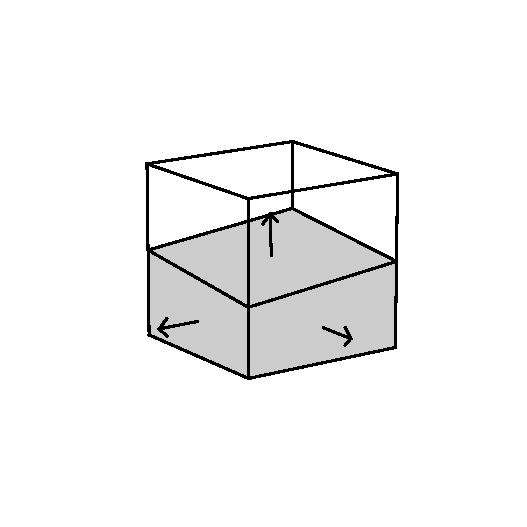
\includegraphics[width=19pc,angle=0]{./figures/cell_diagram.eps}\\
  \caption{C grid cell with cloud surface.}\label{fig:cell_diagram}
\end{figure}

\begin{figure}[t]
  \noindent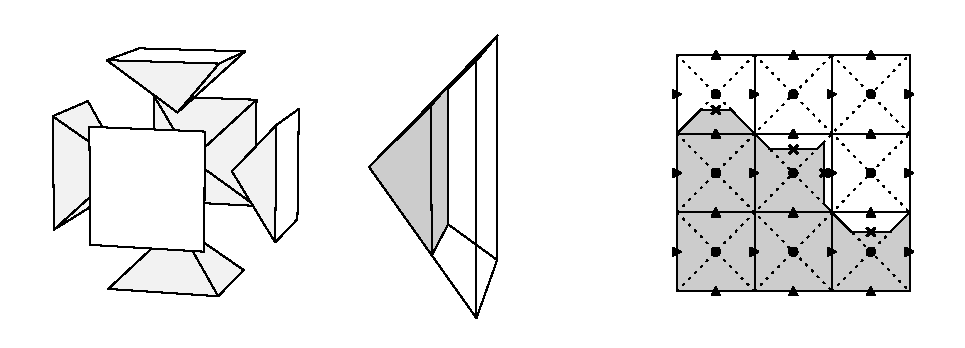
\includegraphics[width=40pc,angle=0]{./figures/pyramid_scheme.eps}\\
  \caption{Schematic representaiton of our pyramid interpolation 
scheme.}\label{fig:pyramid_scheme}
\end{figure}

\begin{figure}[t]
  \noindent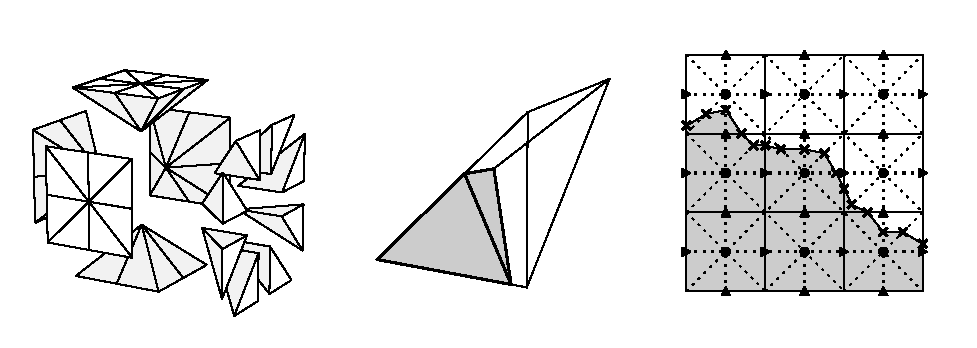
\includegraphics[width=40pc,angle=0]{./figures/tetrahedral_scheme.eps}\\
  \caption{Schematic representaiton of our tetrahedron interpolation 
scheme.}\label{fig:tetrahedral_scheme}
\end{figure}

\begin{figure}[t]
  \noindent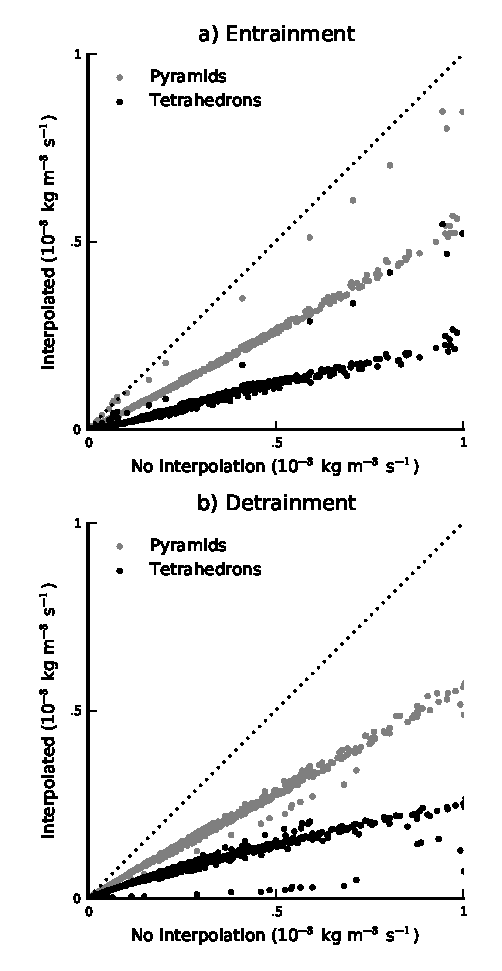
\includegraphics[width=19pc,angle=0]{./figures/effect_of_interpolation.eps}\\
  \caption{Effect of surface interpolation on calculation of a) entrainment and 
b) detrainment.}\label{fig:effect_of_interpolation}
\end{figure}

\begin{figure}[t]
  \noindent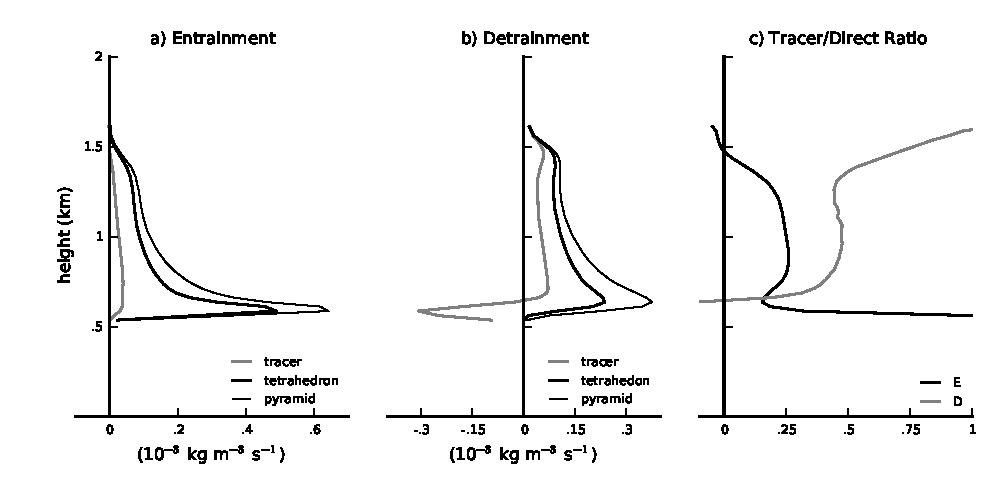
\includegraphics[width=40pc,angle=0]{./figures/direct_vs_tracer_core.eps}\\
  \caption{Comparison of entrainment rates calculated using a) our direct method 
using pyramid interpolation, b) using the conserved bulk tracer method, and 
c) the ratio of the two methods.}\label{fig:direct_vs_tracer}
\end{figure}

\begin{figure}[t]
  \noindent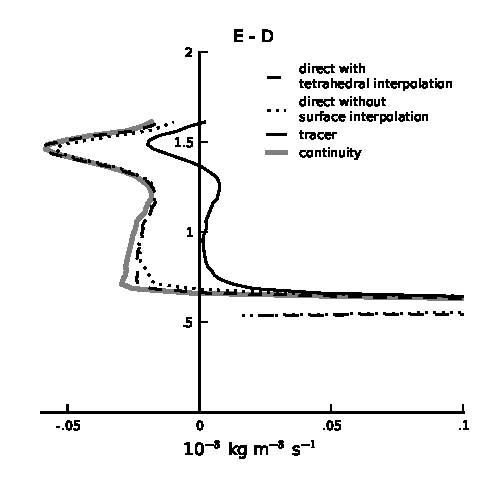
\includegraphics[width=19pc,angle=0]{./figures/E_minus_D_core.eps}\\
  \caption{Entrainment minus Detrainment calculated for...}\label{fig:E_minus_D}
\end{figure}

\begin{figure}[t]
  \noindent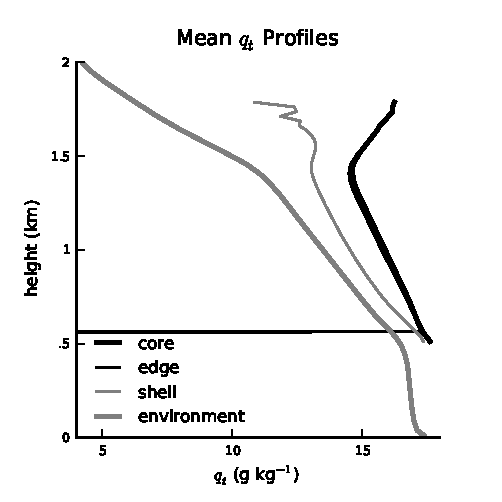
\includegraphics[width=19pc,angle=0]{./figures/shell_edge_profiles_core.eps}\\
  \caption{Height profiles of $q_t$ in the cloud core, core edge, core shell, 
and environment.}\label{fig:shell_edge_profiles}
\end{figure}

\begin{figure}[t]
  \noindent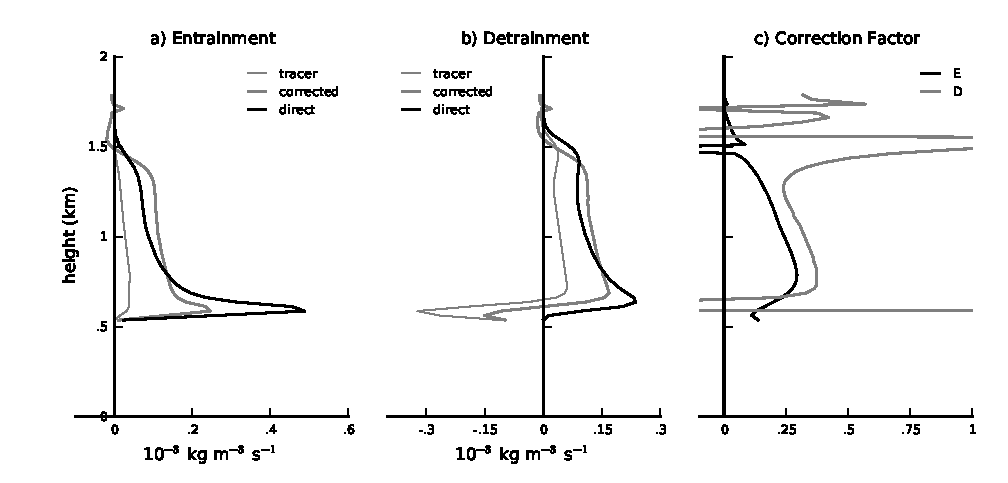
\includegraphics[width=40pc,angle=0]{./figures/corrected_entrainment_core.eps}\\
  \caption{Comparison of a) ratio of direct to tracer entrainment, and b) ratio 
of mean cloud-environment bulk tracer differences to differences at the cloud 
edge.}\label{fig:corrected_entrainment}
\end{figure}


\begin{figure}[t]
  \noindent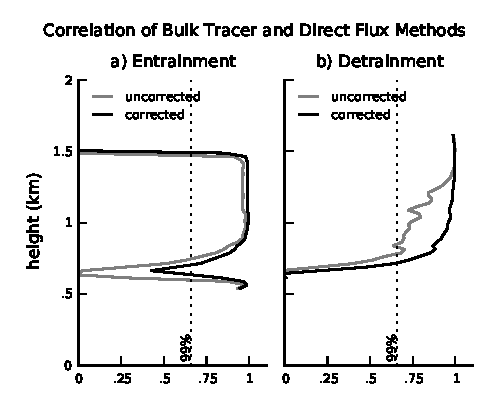
\includegraphics[width=19pc,angle=0]{./figures/correlations_core.eps}\\
  \caption{Correlation between a) entrainment and b) detrainment calculated 
using conserved bulk tracers and direct entrainment calculations with 
tetrahedral interpolation.}\label{fig:correlations}
\end{figure}

\begin{figure}[t]
  \noindent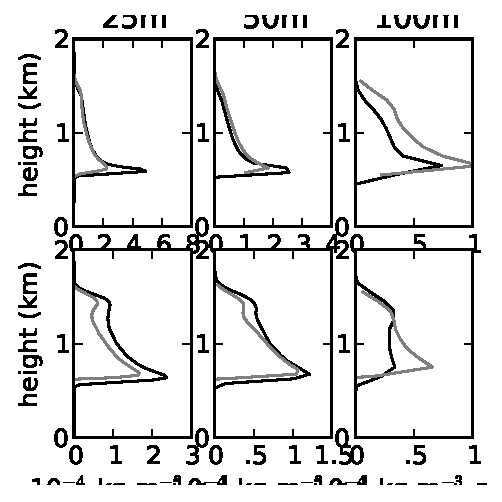
\includegraphics[width=40pc,angle=0]{./figures/resolution_dependence_core.eps}\\
  \caption{Dependance of direct and corrected tracer entrainment on model 
grid resolution.}\label{fig:resolution_dependence}
\end{figure}



%%%%%%%%%%%%%%%%%%%%%%%%%%%%%%%%%%%%%%%%%%%%%%%%%%%%%%%%%%%%%%%%%%%%%
% TABLES
%%%%%%%%%%%%%%%%%%%%%%%%%%%%%%%%%%%%%%%%%%%%%%%%%%%%%%%%%%%%%%%%%%%%%
%\begin{table}[t]
%\caption{This is a sample table caption and table layout.  Enter as many tables as
%  necessary at the end of your manuscript. Table from Lorenz (1963).}\label{t1}
%\begin{center}
%\begin{tabular}{ccccrrcrc}
%\hline\hline
%$N$ & $X$ & $Y$ & $Z$\\
%\hline
% 0000 & 0000 & 0010 & 0000 \\
% 0005 & 0004 & 0012 & 0000 \\
% 0010 & 0009 & 0020 & 0000 \\
% 0015 & 0016 & 0036 & 0002 \\
% 0020 & 0030 & 0066 & 0007 \\
% 0025 & 0054 & 0115 & 0024 \\
%\hline
%\end{tabular}
%\end{center}
%\end{table}
%
\end{document}
